\documentclass[11pt]{article}

\usepackage{extras} % Se extras.sty

\DeclareUnicodeCharacter{00A4}{ }

\begin{document}
\begin{titlepage}
\begin{center}

{\Large\bfseries TSEA56 - Kandidatprojekt i elektronik \\ LIPS Systemskiss}

\vspace{5em}

Version 1.0

\vspace{5em}
Grupp 4 \\
\begin{tabular}{rl}
Hynén Ulfsjöö, Olle&\verb+ollul666+
\\
Wasteson, Emil&\verb+emiwa068+
\\
Tronje, Elena&\verb+eletr654+
\\
Gustafsson, Lovisa&\verb+lovgu777+
\\
Inge, Zimon&\verb+zimin415+
\\
Strömberg, Isak&\verb+isast763+
\\
\end{tabular}

\vspace{5em}
\today

\vspace{16em}
Status
\begin{longtable}{|l|l|l|} \hline

Granskad & OHU & 2016-02-16 \\ \hline
Godkänd & - & - \\ \hline
 
\end{longtable}

\end{center}
\end{titlepage}

\pagebreak
\begin{center}

\section*{PROJEKTIDENTITET}
2016/VT, Undsättningsrobot Gr. 4

Linköpings tekniska högskola, ISY
\vspace{5em}
\begin{center}

\begin{tabular}{|l|l|l|l|} \hline
\textbf{Namn} & \textbf{Ansvar} & \textbf{Telefon} & \textbf{E-post}  \\ \hline 
Isak Strömberg (IS) & Projektledare & 073-980 38 50 & isast763@student.liu.se \\ \hline
Olle Hynén Ulfsjöö (OHU)& Dokumentansvarig & 070-072 91 84 & ollul666@student.liu.se \\ \hline
Emil Wasteson (EW) & Hårdvaruansvarig & 076-836 61 66 & emiwa068@student.liu.se \\ \hline
Elena Tronje (ET) & Mjukvaruansvarig & 072-276 92 93 & eletr654@student.liu.se \\ \hline
Zimon Inge (ZI)& Testansvarig & 070-171 35 18 & zimin415@student.liu.se \\ \hline
Lovisa Gustafsson (LG) & Leveransansvarig & 070-210 32 53 & lovgu777@student.liu.se \\ \hline
\end{tabular}

\end{center}

E-postlista för hela gruppen: isast763@student.liu.se

\vspace{5em}
Kund: ISY, Linköpings universitet \\
tel: 013-28 10 00, fax: 013-13 92 82 \\
Kontaktperson hos kund: Mattias Krysander \\
tel: 013-28 21 98, e-post: matkr@isy.liu.se \\

\vspace{5em}
Kursansvarig:  Tomas Svensson\\
tel: 013-28 13 68, e-post: tomass@isy.liu.se \\
Handledare: Peter Johansson \\
tel: 013-28 13 45, e-post: peter.a.johansson@liu.se
\end{center}
\pagebreak

\tableofcontents

\pagebreak
\section*{Dokumenthistorik}
\begin{table}[h]
\begin{tabular}{|l|l|l|l|l|} \hline

\textbf{Version} & \textbf{Datum} & \textbf{Utförda förändringar} & \textbf{Utförda av} & \textbf{Granskad} \\ \hline
0.1 & 2016-02-12 &  Första utkastet & Grupp 4 & OHU \\ \hline
1.0 & 2016-02-16 &  Andra utkastet & Grupp 4 & OHU \\ \hline
\end{tabular}
\end{table}

\pagebreak
\pagenumbering{arabic}

\begin{flushleft}

\section{Inledning}
Denna systemskiss utgör en del av förarbetet i kandidatprojektet TSEA56. På uppdrag av beställaren ska systemskissen ge en detaljerad beskrivning av produkten och dess delsystem. Dokumentet inleds med en grov beskrivning av produkten, därefter följer en mer detaljerad beskrivning på modulnivå.
\subsection{Syfte och mål}
Syftet med projektet är att bygga en undsättningsrobot på prototypnivå. Roboten ska autonomt kunna utforska en \textit{simulerad} grotta och finna en nödställd. Parallellt med sökandet ska roboten kunna kommunicera med en extern datormodul där en karta av grottan successivt ritas upp. När den nödställde är funnen ska en optimerande algoritm beräkna den kortaste vägen dit. Denna väg ska sedan användas när roboten ska förse den nödställde med någon förnödenhet. Dessa krav finns specificerade i kravspecifikationen, se appendix A.

\pagebreak
\section{Översikt av systemet}
Roboten i sin miljö finns illustrerad i figur \ref{system}. Kommunikationen med datormodulen sker åt båda hållen och via Bluetooth\textsuperscript{\circledR}. Roboten ska dock även klara sitt uppdrag utan kommunikation med datormodulen. Det vill säga att kartläggning, styrning och optimering av kortaste väg sker lokalt hos roboten. Banan är uppbyggd enligt banspecifikationen och uppdraget utförs enligt tävlingsreglerna, se appendix C.
\begin{figure}[htbp]
\centering
\noindent\resizebox{.8\linewidth}{!}{
	
\documentclass[border=10px]{standalone}
\usepackage{tikz}
\usetikzlibrary{patterns}
\usetikzlibrary{shapes.arrows}
\usepackage{amssymb}
\usetikzlibrary{calc}
\usepackage{verbatim}
\usetikzlibrary{decorations.pathmorphing}

\begin{document}
	
\begin{tikzpicture}[scale=1,rotate=0]
		
	%Base
	\draw[thick, draw=black, fill=gray!10] (0,0) rectangle (6,10);

	%Wheels
	\draw[thick, pattern=north west lines, pattern color=black] (-.5,1) 		rectangle (0,2.5);
	\draw[thick, pattern=north west lines, pattern color=black] (-.5,7.5) 	rectangle (0,9);
	\draw[thick, pattern=north west lines, pattern color=black] (6,1) 		rectangle (6.5,2.5);
	\draw[thick, pattern=north west lines, pattern color=black] (6,7.5) 		rectangle (6.5,9);
	
	%Sensors
	\draw[thick, draw=black, fill=white]		(-.25,.25) 		rectangle 	(.5,.75);
	\draw[thick, draw=black, fill=white] 	(-.25,9.25) 		rectangle 	(.5,9.75);
	\draw[thick, draw=black, fill=white] 	(5.5,.25) 		rectangle 	(6.25,.75);
	\draw[thick, draw=black, fill=white] 	(5.5,9.25) 		rectangle 	(6.25,9.75);
	\draw[thick, draw=black, fill=white] 	(1.5,10.25) 		rectangle 	(4.5,9.5);
	\draw[thick, draw=black]				 	(2.5,9.5)			--		  	(2.5,10.25);
	\draw[thick, draw=black]					(3.5,9.5) --++ (0,.75);
	
	%Gripklo
	\draw[thick, draw=black, <-] (3,10.25) --++ (0,.72) node[above] {Gripklo};
	
	%Lidar lite
	\draw[thick, draw=black, <-] 			(1.5,10.25)  		--+ 		  	(135:1) node[above, align=center] {\verb+LIDAR-Lite v2+ \\ med servo};
	%Identifierare av nödställd
	\draw[thick, draw=black, <-]				(4.5,10.25)		--+			(45:1)  node[above] {\verb+IRM-8601-S+};
	
	%IR sensorer
	\draw[thick, draw=black, <-]				(-.25, 9.75) 	--+			(135:1) node[above] {\verb+GP2D120+};
	\draw[thick, draw=black, <-]				(-.25, .25) 		--+			(225:1) node[below] {\verb+GP2D120+};
	\draw[thick, draw=black, <-]				(6.25, 9.75) 	--+			(45:1) node[above] {\verb+GP2D120+};
	\draw[thick, draw=black, <-]				(6.25, .25) 		--+			(315:1) node[below] {\verb+GP2D120+};
	
	\draw[thick, draw=black, fill=white]					(2.5,4.5)		rectangle	(3.5,5.5);
	
	%Gyro
	\draw[thick, draw=black, <-] (3.5,5) --++ (.25,0) node[rotate=270, above] {\verb+MLX90609+};
	
	%Arrows and text
	%\draw[thick, ->]  (3,11) node[left, align=center] {\verb+LIDAR-Lite v2+ \\ + detektor av nödställd} -- (3,10.25);
	%\draw[thick, <->] (0.5,0.5)  --  (5.5,0.5) node[left=-14pt,midway, fill=gray!10] {\verb+GP2D120+};
	%\draw[thick, <->] (0.5,9.5) -- (3,9) node[right=-14pt,fill=gray!10] {\verb+GP2D120+} -- (5.5,9.5);
	%\draw[thick, ->] (4.5,5) node[above] {\verb+MPU-6500+} -- (3.5,5);
	
	%Sensormodul
	\node (sensormodul) at (3,6.75) [thick, draw=black, minimum width=3cm, minimum height=1.5cm, align=center, fill=white] {Sensormodul \\ \verb+ATmega1284p+};
	
	%Huvudmodul
	\node (huvudmodul) at (3,3.25) [thick, draw=black, minimum width=3cm, minimum height=1.5cm, align=center, fill=white] {Huvudmodul \\ \verb+ATmega1284p+};
	
	%Styrmodul
	\node (styrmodul) at (3,1.25) [thick, draw=black, minimum width=3cm, minimum height=1.5cm, align=center, fill=white] {Styrmodul \\ \verb+ATmega1284p+};
	
	%I2C-buss
	\draw[thick, draw=teal] ($(sensormodul.north east) + (.25,0)$) -- ($(styrmodul.south east) + (.25,0)$);
	\draw[thick, draw=teal] ($(sensormodul.north east) + (.5,0)$) -- ($(styrmodul.south east) + (.5,0)$);
	\node (i2c) at ($(sensormodul.north east) + (0.375,.25)$) [text=teal] {\small I\textsuperscript{2}C};
	
	\draw[thick, draw=teal, fill=teal] ($(sensormodul.south east) + (0,.25)$) --+ (.25,0) circle [radius=.05cm];
	\draw[thick, draw=teal, fill=teal] ($(sensormodul.south east) + (0,.5)$) --+ (.5,0) circle [radius=.05cm];
	
	\draw[thick, draw=teal, fill=teal] ($(huvudmodul.south east) + (0,.25)$) --+ (.25,0) circle [radius=.05cm];
	\draw[thick, draw=teal, fill=teal] ($(huvudmodul.south east) + (0,.5)$) --+ (.5,0) circle [radius=.05cm];
	
	\draw[thick, draw=teal, fill=teal] ($(styrmodul.south east) + (0,.25)$) --+ (.25,0) circle [radius=.05cm];
	\draw[thick, draw=teal, fill=teal] ($(styrmodul.south east) + (0,.5)$) --+ (.5,0) circle [radius=.05cm];
	
	%Koppling till sensormodul
	\draw[thick, draw=violet] (.5,9.5) --++ (.25,0) --++ (0,-2.5) --++ (0.75,0) ;
	\draw[thick, draw=violet] (.5,.5) --++ (.25,0) --++ (0,6.25) --++ (0.75,0);
	
	\draw[thick, draw=violet] (5.5,9.5) --++ (-.25,0) --++ (0,-2.5) --++ (-0.75,0);
	\draw[thick, draw=violet] (5.5,.5) --++ (-.25,0) --++ (0,6.25) --++ (-0.75,0);
	
	\draw[thick, draw=violet] (2,9.5) --++ (0,-2);
	\draw[thick, draw=violet] (4,9.5) --++ (0,-2);
	
	\draw[thick, draw=violet] (sensormodul.south) --++ (0,-.5);
	
	%Kopplingar till styrmodul
	\draw[thick, draw=olive] (styrmodul.east) --++ (1.5,0);
	\draw[thick, draw=olive] (styrmodul.west) --++ (-1.5,0);
	\draw[thick, draw=olive] ($(styrmodul.east) + (0,.25)$) --++ (1,0) --++ (0,6.25) --++ (.5,0);
	\draw[thick, draw=olive] ($(styrmodul.west) + (0,.25)$) --++ (-1,0) --++ (0,6.25) --++ (-.5,0);
	\draw[thick, draw=olive] (3,9.5) --++ (0,-1.75) --++ (-1.75,0) --++ (0,-6) --++ (.25,0);
	
	%Bluetooth
	\draw[thick, draw=black] (huvudmodul.east) --++ (2,0) node[right,minimum width=.75cm, minimum height=1cm, draw=black] (bt) {
\includegraphics{bluetooth}};
	
	\node (bt2) at ($(bt) + (2,0)$) [thick, draw=black, minimum width=.75cm, minimum height=1cm] {
\includegraphics{bluetooth}};
	
	\draw[thick, ->,line join=round,decorate, decoration={
    												snake,
    												segment length=5,
    												amplitude=1,
    												post=lineto,
    												post length=1pt}] 
    		($(bt.east) + (5pt,5pt)$) -- ($(bt2.west) + (-5pt,5pt)$);
    		
    \draw[thick, ->,line join=round,decorate, decoration={
    												snake,
    												segment length=5,
    												amplitude=1,
    												post=lineto,
    												post length=1pt}] 
    		 ($(bt2.west) + (-5pt,-5pt)$) -- ($(bt.east) + (5pt,-5pt)$);
    		 
    \draw[thick, draw=black] (bt2.east) --++ (.5,0) node[right, minimum width=3cm, minimum height=1.5cm, draw=black, fill=white] {Datormodul};
    
    \draw[thick, draw=black] ($(sensormodul.south west) + (.25,0)$) --++ (0,-2) node[midway, above, sloped] {\small avbrott};
    
    \draw[thick, draw=black] ($(styrmodul.north west) + (.25,0)$) -- ($(huvudmodul.south west) + (.25,0)$) node[right, midway] {\small avbrott};
	
	\end{tikzpicture}
	
\end{document}  
}
	\caption{Översikt av systemet \label{system}}	
\end{figure}


\subsection{Beskrivning av systemet}
Roboten navigerar själva banan med hjälp av flertal sensorer, dessa är specificerade i \mbox{avsnitt \ref{sec:sensormodul}}. En regleringsmodell ser till att roboten färdas i mitten av korridorerna och kan ta svängar utan att stöta mot väggar. Under färden ska roboten autonomt kartlägga och finna den kortaste vägen mellan ingången och den nödställde. Ifall roboten även är uppkopplad mot datormodulen ska mjukvara på datorn successivt rita upp en karta och kunna presentera utvalda mätvärden i realtid. När den kortaste vägen är funnen ska roboten använda denna rutt för att förse den nödställde med en förnödenhet. Förnödenheten transporteras med hjälp av robotens gripklo.

\subsection{Delsystem}
Delsystemen och dess ingående komponenter finns beskrivna nedan. \\*
\vspace{1em}
\begin{minipage}{\textwidth}
\begin{description}
	\item[Delsystem 1 - Huvudmodul] \hfill \\
	Mikroprocessor \\
	Brytare för autonomt/manuellt-läge \\
	Bluetooth\textsuperscript{\circledR} sändare/mottagare
	\item[Delsystem 2 - Sensormodul] \hfill \\
	Mikroprocessor \\
	Sensorer
	\item[Delsystem 3 - Styrmodul] \hfill \\
	Mikroprocessor \\
	Motorer till hjul och gripklo \\
	LCD-display
	\item[Delsystem 4 - Datormodul] \hfill \\
	Dator \\
	GUI \\
	Bluetooth\textsuperscript{\circledR} sändare/mottagare
\end{description}
\end{minipage}

Ovanstående mikroprocessorer är av typ \verb+ATmega**+ där versionen bestäms i ett senare skede. Sensorerna består av avståndsmätare, vinkelhastighets-sensorer och identifierare av nödställd. 
\subsection{Kommunikation mellan delsystem}
Kommunikationen mellan mikroprocessorerna sker med hjälp av en I\textsuperscript{2}C-buss enligt figur \ref{communication}. Mellan huvudmodulen och datormodulen sker kommunikationen via Bluetooth\textsuperscript{\circledR}.

\begin{figure}[htbp]
\noindent\resizebox{.97\textwidth}{!}{
	\documentclass[border=20pt]{standalone}
\usepackage{tikz}
\usetikzlibrary{positioning}
\usetikzlibrary{calc}
\usetikzlibrary{decorations.pathmorphing}
\usepackage{amssymb}
\usetikzlibrary{shapes,arrows}

\begin{document}
	\begin{tikzpicture}[scale=1]
		
		\tikzset{every node/.style={thick, draw=black, align=center, minimum height=40pt, text width=100pt, minimum width=100pt}}
		\node(datormodul) {Datormodul};
		\node[right=10pt of datormodul,minimum height=20pt, minimum width=10pt,text width=10pt] (bt1) {
\includegraphics{bluetooth}};
		
		\node[right=40pt of bt1,minimum height=20pt, minimum width=10pt,text width=10pt] (bt2) {
\includegraphics{bluetooth}};
		
		\node[right=10pt of bt2] 			(huvudmodul) 	{Huvudmodul};
		\node[below=-10pt of huvudmodul,draw=none] (master) {\textit{master}};
		\node[right=10pt of huvudmodul] 		(sensormodul) 	{Sensormodul};
		\node[below=-10pt of sensormodul,draw=none] (slave1) {\textit{slav}};
		\node[right=10pt of sensormodul] 	(styrmodul) 		{Styrmodul};
		\node[below=-10pt of styrmodul,draw=none] (slave2) {\textit{slav}};
		
		\coordinate (sclStart) 	at ($(huvudmodul.north west) + (0,20pt)$);
		\coordinate (sclEnd)		at ($(styrmodul.north east)  + (0,20pt)$);
		
		\coordinate (sdaStart)  at ($(sclStart) + (0,20pt)$);
		\coordinate (sdaEnd)		at ($(sclEnd)	+ (0,20pt)$);
		
		\coordinate (vddStart)  at ($(sdaStart) + (0,40pt)$);
		\coordinate (vddEnd)		at ($(sdaEnd)	+ (0,40pt)$);
		
		\draw[thick] (sclStart) -- (sclEnd) node [right,draw=none,text width=0,minimum width=0] {SCL};
		\draw[thick] (sdaStart) -- (sdaEnd) node [right,draw=none,text width=0,minimum width=0] {SDA};
		\draw[thick] (vddStart) -- (vddEnd) node [right,draw=none,text width=0,minimum width=0] {$V_{dd}$};
		
		\draw[thick] (datormodul.east) -- (bt1.west);
		
		\draw[thick, ->,line join=round,decorate, decoration={
    												snake,
    												segment length=5,
    												amplitude=1,
    												post=lineto,
    												post length=1pt}] 
    		($(bt1.east) + (5pt,5pt)$) -- ($(bt2.west) + (-5pt,5pt)$);
    		
    	\draw[thick, ->,line join=round,decorate, decoration={
    												snake,
    												segment length=5,
    												amplitude=1,
    												post=lineto,
    												post length=1pt}] 
    		 ($(bt2.west) + (-5pt,-5pt)$) -- ($(bt1.east) + (5pt,-5pt)$);
    		 
    	\draw[thick] (bt2.east) -- (huvudmodul.west);
    	
    	\draw[thick,fill=black] ($(huvudmodul.north) + (-10pt,0)$) -- ($(huvudmodul.north) + (-10pt,20pt)$) circle [radius=2pt];
    	\draw[thick,fill=black] ($(huvudmodul.north) + (+10pt,0)$) -- ($(huvudmodul.north) + (+10pt,40pt)$) circle [radius=2pt];
    	
    	\draw[thick,fill=black] ($(sensormodul.north) + (-10pt,0)$) -- ($(sensormodul.north) + (-10pt,20pt)$) circle [radius=2pt];
    	\draw[thick,fill=black] ($(sensormodul.north) + (+10pt,0)$) -- ($(sensormodul.north) + (+10pt,40pt)$) circle [radius=2pt];
    	
    	\draw[thick,fill=black] ($(styrmodul.north) + (-10pt,0)$) -- ($(styrmodul.north) + (-10pt,20pt)$) circle [radius=2pt];
    	\draw[thick,fill=black] ($(styrmodul.north) + (+10pt,0)$) -- ($(styrmodul.north) + (+10pt,40pt)$) circle [radius=2pt];
    	
    	\draw[thick,fill=black] ($(sensormodul.north east) + (-5pt,20pt)$) circle [radius=2pt] -- ($(sensormodul.north east) + (-5pt,80pt)$) circle [radius=2pt];
    	\draw[thick,fill=black] ($(styrmodul.north west) + (5pt,40pt)$) circle [radius=2pt] -- ($(styrmodul.north west) + (5pt,80pt)$) circle [radius=2pt];
    	\draw[thick,draw=black,fill=white] ($(styrmodul.north west) + (2pt,50pt)$) rectangle ($(styrmodul.north west) + (8pt,70pt)$);
		\draw[thick,draw=black,fill=white] ($(sensormodul.north east) + (-8pt,50pt)$) rectangle ($(sensormodul.north east) + (-2pt,70pt)$) node [below left=-10pt and 20pt,draw=none,minimum width=0, text width = 0pt] {$R_p$};
		
		\draw[thick, ->] ($(sensormodul.south) + (+40pt,0)$) -- ($(sensormodul.south) + (40pt,-30pt)$) -- ($(huvudmodul.south) + (40pt,-30pt)$) -- ($(huvudmodul.south) + (40pt,0)$);
		\draw[thick, ->] ($(styrmodul.south) + (+40pt,0)$) -- ($(styrmodul.south) + (40pt,-40pt)$) -- node [midway,below,minimum height=20pt, draw=none] {Avbrott}($(huvudmodul.south) + (30pt,-40pt)$) -- ($(huvudmodul.south) + (30pt,0)$);
	\end{tikzpicture}
\end{document}}
	\caption{Intermodulär kommunikation \label{communication}}
\end{figure}

\pagebreak
\section{Delsystem 1 - Huvudmodul}
\label{sec:huvudmodul}
Genom delsystem 1, tillika systemets huvudmodul, kommer all komunikation mellan roboten och en extern datormodul att ske. Systemkonstruktionen för roboten är konstruerad på ett sådant vis att huvudmodulen kommer att verka som överordnad processorenhet (\emph{master}) i den tvåtrådsbuss som förbinder robotens olika delsystem. 
\subsection{Strömbrytare}
Robotens strömbrytare ska vara kopplad till en av huvudmodulens avbrottsingångar. När denna triggas så ska processorerna i huvudmodulen, sensormodulen samt styrmodulen gå in i viloläge. Anledningen till att dessa ska inträda i viloläge, snarare än att bryta strömförsörjningen helt, är främst för att bespara användaren att ånyo tvingas kalibrera sensorerna vid varje uppstart.
\subsection{Brytare för autonomt respektive manuellt läge}
Brytaren mellan autonomt och manuellt körläge tillåter användaren att välja mellan robotens två körlägen. Liksom strömbrytaren ska även denna kopplas till en av huvudmodulens avbrottsingångar. Brytaren ska även vara studsfri för att säkerställa att systemet ingår det körläge som användaren önskat.
\subsection{Bluetooth\textsuperscript{\circledR} sändare/mottagare} \label{bluetooth} 
Kommunikationen mellan den externa datormodulen och roboten kommer att ske via Bluetooth\textsuperscript{\circledR}. Det data som sensormodulen har samlat in (och bearbetat) kommer att kommuniceras till huvudenheten, vilken kommer att vidarebefordra mätdata från banan till datormodulen. Vid manuellt körläge ska huvudmodulen i sin tur mottaga styrkommandon från datormodulen. Används Firefly vesion 1.2 kan överföringen ske till en hastighet av 723.1 kbit/s, vilket är mer än tillräcklig överföringshastighet för en ATmega-processor av den sort som planeras användas i roboten.


\pagebreak
\section{Delsystem 2 - Sensormodul}
\label{sec:sensormodul}
Sensormodulens uppdrag är att kommunicera med både sensorerna och huvudmodulen. Mätdata samplas med konstant frekvens och konverteras därefter till motsvarande SI-enhet. För avståndssensorerna innebär detta att den analoga inspänningen konverteras till ett digitalt värde i enheten meter.

Den främre avståndssensorn (laser-sensorn) placeras på ett roterande servo så att den kan \emph{scanna} korridoren roboten befinner sig i. Detta förutsätter att servot går att styra så att vinkelutslaget går att beräkna med godtycklig precision. Tillåter inte servot en sådan styrning placeras laser-sensorn så att den konstant pekar rakt framåt.

Vinkelhastighets-sensorerna används för att beräkna vinkelutslag då roboten tar en sväng. Mätdatan behöver därför integreras under ett tidsintervall och konverteras till en vinkel. Hur den nödställde ska representeras är ännu inte fastställt. Förslagsvis används en IR-fyr i kombination med en IR-sensor. Sensormodulens uppdrag blir då att ta beslutet om när den nödställde är funnen.


\subsection{Sensorer}
De sensorer som används är följande,
\begin{description}
	\item[Avstånd] \hfill \\
	4 x IR-sensor \verb+GP2D120+ (4 cm till 30 cm) \\
	1 x Laser-sensor \verb+LIDAR-Lite v2+ (0 till 40 m) \\
	\item[Vinkelhastighet] \hfill \\
	1 x Gyro/accelerometer \verb+MPU-6500+ 
	\item[Identifierare av nödställd] \hfill \\
	1 x IR-detektor \verb+IRM-8601-S+
\end{description}
och är placerade enligt figur \ref{sensors}. 

\begin{figure}[htbp]
\centering
\noindent\resizebox{.8\textwidth}{!}{
	\documentclass[border=10px]{standalone}
\usepackage{tikz}
\usetikzlibrary{patterns}
\usetikzlibrary{shapes.arrows}
\usepackage{amssymb}
\usetikzlibrary{calc}
\usepackage{verbatim}
\begin{document}
	
\begin{tikzpicture}[scale=1,rotate=90]
		
	%Base
	\draw[thick, draw=black, fill=gray!10] (0,0) rectangle (6,10);

	%Wheels
	\draw[thick, pattern=north west lines, pattern color=black] (-.5,1) 		rectangle (0,2.5);
	\draw[thick, pattern=north west lines, pattern color=black] (-.5,7.5) 	rectangle (0,9);
	\draw[thick, pattern=north west lines, pattern color=black] (6,1) 		rectangle (6.5,2.5);
	\draw[thick, pattern=north west lines, pattern color=black] (6,7.5) 		rectangle (6.5,9);
	
	%Sensors
	\draw[thick, draw=black, fill=white] (-.25,.25) 		rectangle (.5,.75);
	\draw[thick, draw=black, fill=white] (-.25,9.25) 	rectangle (.5,9.75);
	\draw[thick, draw=black, fill=white] (5.5,.25) 		rectangle (6.25,.75);
	\draw[thick, draw=black, fill=white] (5.5,9.25) 		rectangle (6.25,9.75);
	\draw[thick, draw=black, fill=white] (2,10.25) 		rectangle (4,9.5);
	\draw[thick, draw=black, fill=white] (2.5,4) 		rectangle (3.5,6);
	
	%Arrows and text
	\draw[thick, ->]  (3,11) node[left, align=center] {\verb+LIDAR-Lite v2+ \\ + detektor av nödställd} -- (3,10.25);
	\draw[thick, <->] (0.5,0.5)  --  (5.5,0.5) node[left=-14pt,midway, fill=gray!10] {\verb+GP2D120+};
	\draw[thick, <->] (0.5,9.5) -- (3,9) node[right=-14pt,fill=gray!10] {\verb+GP2D120+} -- (5.5,9.5);
	\draw[thick, ->] (4.5,5) node[above] {\verb+MLX90609+} -- (3.5,5);
	\end{tikzpicture}
	
\end{document}	}
	\caption{Sensorplacering \label{sensors}}
\end{figure}

IR-sensorerna och detektorn har endast en analog utspänning och behöver därför passera en ADC. Den interna ADC:n i ATmega används tillsammans med en multiplexer för att avläsa sensorvärdena med godtycklig frekvens. 

Både laser-sensorn och gyro/accelerometern har inbyggt stöd för protokollet I\textsuperscript{2}C och kopplas enklast upp på en sub-I\textsuperscript{2}C-buss alternativt analogt in på multiplexern. Frekvensen med vilket avläsningarna görs bestäms senare i projektet. Faktorer som ADC:ns konverteringstid samt accelerometerns precision kommer att påverka samplingsfrekvensen och kan bestämmas först under testkörningar. 

\subsection{Kommunikation med huvudmodul}
Sensormodulen kommunicerar med huvudmodulen enligt den I\textsuperscript{2}C-buss som är definierad i avsnitt \ref{sec:huvudmodul}. Eftersom sensormodulen är \emph{slave} i sammanhanget så anropar den huvudmodulen via ett avbrott när information ska skickas. Informationen som skickas är avstånd till den främre väggen, avstånd till sidovägg, vinkel mot sidovägg och eventuellt vinkelutslag, se figur \ref{measurements}. 

\begin{figure}[htbp]
\centering

\noindent\resizebox{.5\textwidth}{!}{
	\documentclass[border=10px]{standalone}
\usepackage{tikz}
\usetikzlibrary{patterns}
\usetikzlibrary{shapes.arrows}
\usepackage{amssymb}
\usetikzlibrary{calc}
\usepackage{verbatim}
\usetikzlibrary{intersections}
\usetikzlibrary{decorations.pathreplacing}
\begin{document}
	
	\begin{tikzpicture}[scale=1]
		
		%Sides
		\path [name path=left, draw=black,thick] (0,0) -- (0,20);
		\path [name path=right, draw=black,thick] (15,0) -- (15,20);	

		%Robot
		\node (robot) at (7.5,10) [draw, thick, minimum width=6cm, minimum height=10cm,align=center,rotate=30,fill=gray!10] {};
		\node [rotate=30] at ($(robot.north) + (-60:2cm)$) {\huge Robot};
		\node [rotate=30,minimum width=1cm, minimum height=2cm, fill=white,draw=black] at ($(robot.north) + (-60:5cm)$) {};
		\coordinate (start1) at ($(robot.north west) + (-60:.5cm)$);
		\coordinate (start2) at ($(robot.south west) + (120:.5cm)$);
		\coordinate (start3) at ($(robot.north east) + (-60:.5cm)$);
		\coordinate (start4) at ($(robot.south east) + (120:.5cm)$);
		
		\coordinate (middle1) at ($(robot.north west) + (-60:5cm)$);
		\coordinate (middle2) at ($(robot.north east) + (-60:5cm)$);
		
		\path [name path=path1,overlay,rotate=30] (start1) -- +(-20cm,0cm);
		\path [name path=path2,overlay,rotate=30] (start2) -- +(-20cm,0cm);
		\path [name path=path3,overlay,rotate=30] (start3) -- +(20cm,0cm);
		\path [name path=path4,overlay,rotate=30] (start4) -- +(20cm,0cm);
		
		\path [name path=middlePath1,overlay,rotate = 30] (middle1) -- +(-20cm,0cm);
		\path [name path=middlePath2,overlay,rotate = 30] (middle2) -- +(20cm, 0cm);
		
		\path [name path=left1, name intersections={of=path1 and left, by=x1},thick, draw=black,dashed] (start1) -- (x1);
		\path [name path=left2, name intersections={of=path2 and left, by=x2},thick, draw=black,dashed] (start2) -- (x2);
		\path [name path=right1, name intersections={of=path3 and right, by=x3},thick, draw=black,dashed] (start3) -- (x3);
		\path [name path=right2, name intersections={of=path4 and right, by=x4},thick, draw=black,dashed] (start4) -- (x4);
		
		\path [name path=int1, name intersections={of=left and middlePath1, by=m1}, thick, draw=black, dashed] (middle1) -- (m1);
		\path [name path=int2, name intersections={of=right and middlePath2, by=m2}, thick, draw=black, dashed] (middle2) -- (m2);
		
		\path [name path=kat1,overlay] (x1) -- +(-60:20cm);
		\path [name path=kat2,overlay] (x4) -- +(120:20cm);
		
		\path [name intersections={of= kat1 and left2, by=x5}, thick, draw=black,dashed] (x1) -- (x5);
		\draw ($(x1) - (0,2cm)$) arc [start angle=-90, end angle=-60, radius=2cm,thick] node [midway, yshift=-1cm] {\huge $\alpha$};
		
		\path [name intersections={of= kat2 and right1, by=x6}, thick, draw=black,dashed] (x4) -- (x6);
		\draw ($(x4) + (0,2cm)$) arc [start angle=-270, end angle=-240, radius=2cm,thick] node [midway, yshift=1cm] {\huge $\alpha$};
		\draw[thick, draw=black, ->,dashed] (robot.north) --+(120:5cm);
		
		\draw [thick, draw=black, ->] ($(robot.north) + (-60:6.5cm)$) arc [start angle=300, end angle=480, radius=1.5cm, thick] node[right=2.2cm] {\huge $\omega$};
		
		\draw [thick, fill=white, rotate=0] ($(robot.north west) + (-60:.75cm) + (-150:0.25cm)$) -- ($(robot.north west) + (-60:.75cm) + (-150:-0.5cm)$) -- ($(robot.north west) + (-60:0.25cm) + (-150:-0.5cm)$) -- ($(robot.north west) + (-60:0.25cm) + (-150:0.25cm)$) -- ($(robot.north west) + (-60:0.75cm) + (-150:0.25cm)$);
		
		\draw [thick, fill=white, rotate=0] ($(robot.north west) + (-60:9.75cm) + (-150:0.25cm)$) -- ($(robot.north west) + (-60:9.75cm) + (-150:-0.5cm)$) -- ($(robot.north west) + (-60:9.25cm) + (-150:-0.5cm)$) -- ($(robot.north west) + (-60:9.25cm) + (-150:0.25cm)$) -- ($(robot.north west) + (-60:9.75cm) + (-150:0.25cm)$);
		
		\draw [thick, fill=white, rotate=0] ($(robot.north east) + (-60:.75cm) + (-150:0.25cm)$) -- ($(robot.north east) + (-60:.75cm) + (-150:-0.5cm)$) -- ($(robot.north east) + (-60:0.25cm) + (-150:-0.5cm)$) -- ($(robot.north east) + (-60:0.25cm) + (-150:0.25cm)$) -- ($(robot.north east) + (-60:0.75cm) + (-150:0.25cm)$);
		
		\draw [thick, fill=white, rotate=0] ($(robot.north east) + (-60:9.75cm) + (-150:0.25cm)$) -- ($(robot.north east) + (-60:9.75cm) + (-150:-0.5cm)$) -- ($(robot.north east) + (-60:9.25cm) + (-150:-0.5cm)$) -- ($(robot.north east) + (-60:9.25cm) + (-150:0.25cm)$) -- ($(robot.north east) + (-60:9.75cm) + (-150:0.25cm)$);
		
		\draw [thick, pattern=north west lines, pattern color=black] ($(robot.north west) + (-60:1cm)$) -- ++(30:-.5) -- ++(120:-1.5cm) -- ++(30:.5) -- +(-60:-1.5);
		\draw [thick, pattern=north west lines, pattern color=black] ($(robot.north west) + (-60:7.5cm)$) -- ++(30:-.5) -- ++(120:-1.5cm) -- ++(30:.5) -- +(-60:-1.5);
		
		\draw [thick, pattern=north west lines, pattern color=black] ($(robot.north east) + (-60:1cm) + (30:.5cm)$) -- ++(30:-.5) -- ++(120:-1.5cm) -- ++(30:.5) -- +(-60:-1.5);
		\draw [thick, pattern=north west lines, pattern color=black] ($(robot.north east) + (-60:7.5cm) + (30:.5cm)$) -- ++(30:-.5) -- ++(120:-1.5cm) -- ++(30:.5) -- +(-60:-1.5);
		
		\draw [thick, fill=white] ($(robot.north) + (30:1cm) + (-60:0.5cm)$) --++(120:0.75cm) --++(210:2cm) --++(-60:0.75cm) --++(30:2cm);
		
		\draw [decorate,decoration={brace,amplitude=10pt},xshift=-10pt,yshift=0pt] ($(robot.north) + (120:5cm) + (30:0.2cm)$) -- +(120:-4.75cm) node [black,midway,xshift=1cm,yshift=0.3cm] {\huge $l$};
		
		\draw [decorate,decoration={brace,amplitude=10pt},xshift=-10pt,yshift=5pt] ($(middle1) +(-60:.2cm)$) -- ($(m1) +(-60:.2cm)$) node [black,midway,xshift=.8cm,yshift=-.5cm] {\huge $l_{\perp}$};
		
	\end{tikzpicture}
	
\end{document}}
	\captionsetup{justification=centering}
	\caption{Sensorerna i arbete, \\ $\alpha$ är vinkeln mot sidovägg, \\ $l$ är avståndet till främre vägg, \\ $\l_{\perp}$ är avständet till sidovägg och \\ $\omega$ vinkelhastigheten}
	\label{measurements}
\end{figure}
\pagebreak
\section{Delsystem 3 - Styrmodul}
Styrmodulen tar emot kommandon från huvudmodulen och verkställer dessa. Det är antingen styrning av chassits motorer för att få roboten att röra på sig, rotera det eventuella lasersensortornet eller att styra gripklon. Kommunikationen sker genom I\textsuperscript{2}C-bussen. Styrmodulen har även LCD-displayer kopplade till sig för att kunna skriva ut valda sensorvärden.
\subsection{Motorer}
Det chassi som roboten byggs på har fyra hjul. Dessa styrs parvis, höger hjulpar respektive vänster hjulpar. Signalerna till respektive sida styr rotationsriktning respektive hastighet. Signalen som styr hastigheten ska vara pulsbreddsmodulerad.
\subsection{LCD-display}
För att skriva ut sensordata på display används den alphanumeriska LCD-displayen \textit{LCD JM162A}. Den har totalt 16 pinnar, där 8 stycken är databitar, 3 stycken för konfiguration (inställning av funktion) och resterande är referenssignaler och strömtillförsel.

\subsection{Gripklo}
Gripklon ska kunna öppnas och stängas på kommando från huvudmodulen. 

\pagebreak
\section{Delsystem 4 - Datormodul}
Datormodulen kommunicerar med robotens huvudmodul via Bluetooth\textsuperscript{\circledR}. Signaler mellan dessa enheter ska kunna skickas åt båda hållen, vilket innebär en sändare och en mottagare på datormodulen. Mot användaren ska det finnas ett program för att se var roboten gör.
\subsection{Bluetooth\textsuperscript{\circledR} sändare/mottagare}
Se avsnitt \ref{bluetooth}.
\subsection{Mjukvara}
Mjukvara till datormodulen utvecklas från grunden. I första hand utvecklas den i Java men upptäcks begränsningar väljs alternativa språk, exempelvis Python eller C\texttt{++}. Användaren ska presenteras en tabell med valda sensorvärden och en karta över utforskad del av banan. Till hjälp för felsökning ska sensorvärden även kunna presenteras i en graf som kontinuerligt uppdateras i realtid. 

Programmet ska även möjliggöra för användaren att styra roboten manuellt med hjälp av tangentbordet. Mjukvaran ska lyssna efter knapptryckningar på piltangenterna och kontinuerligt skicka vilka tangenter som hålls nere till roboten. De kommandon som ska finnas tillgängliga är presenterade i tabell \ref{commands}.

\begin{longtable}{|p{.05\linewidth} p{.05\linewidth} p{.05\linewidth} p{.05\linewidth} c l|}
	\multicolumn{4}{c}{\textbf{Knapptryckning}} & & \multicolumn{1}{l}{\textbf{Översättning}} 	\\ \hline\hline
	$\uparrow$ &  				&  				& 				& = & Kör framåt 				\\ \hline
	$\uparrow$ & $\leftarrow$	&				&				& = & Kör framåt vänster 		\\ \hline
	$\uparrow$ &				& $\rightarrow$	&				& = & Kör framåt höger 			\\ \hline
			   & $\leftarrow$	&				&				& = & Rotera medurs 			\\ \hline
			   &				& $\rightarrow$	&				& = & Rotera moturs 			\\ \hline
			   & $\leftarrow$	&				& $\downarrow$	& = & Kör bakåt vänster 		\\ \hline
			   &				& $\rightarrow$ & $\downarrow$	& = & Kör bakåt höger 			\\ \hline
			   &				&				& $\downarrow$	& = & Kör bakåt 				\\ \hline
	\caption{Knapptryckningar och dess översättning} \label{commands}
\end{longtable}

\pagebreak
\subsection{Grafiskt gränssnitt}
Gränssnittet kommer konstrueras enligt figur \ref{software}.
\begin{figure}[htbp]
\centering
\noindent\resizebox{.5\textwidth}{!}{
	\documentclass[border=10px]{standalone}
\usepackage{tikz}
\usetikzlibrary{patterns}
\usetikzlibrary{shapes.arrows}
\usepackage{amssymb}
\usetikzlibrary{calc}
\usepackage{verbatim}
\usepackage[swedish]{babel}
\begin{document}
	
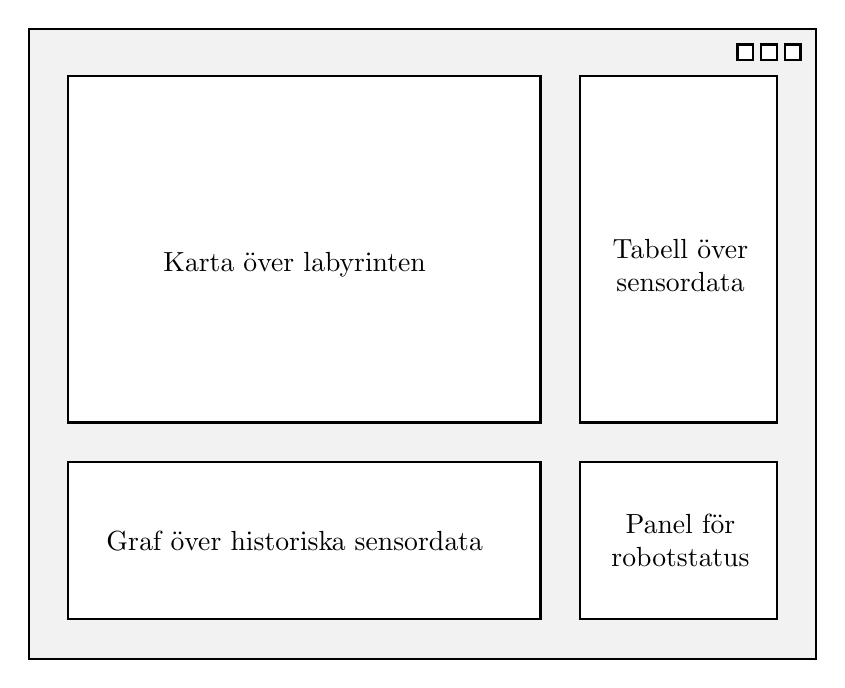
\begin{tikzpicture}[scale=1,rotate=0]
		
	%Frame
	\draw[thick, draw=black, fill=gray!10] (0,0) rectangle (10,8);

	%Exit and minimize
	\draw[thick, draw=black, fill=white] (9.0,7.6) rectangle (9.2,7.8);
	\draw[thick, draw=black, fill=white] (9.3,7.6) rectangle (9.5,7.8);
	\draw[thick, draw=black, fill=white] (9.6,7.6) rectangle (9.8,7.8);
	
	%Map
	\draw[thick, draw=black, fill=white] (0.5,3) rectangle (6.5,7.4);
	\draw  node[left, align=center, text width=5cm] at (6,5) {Karta över labyrinten};
	
	%Table
	\draw[thick, draw=black, fill=white] (7, 3) rectangle (9.5,7.4);
	\draw  node[left, align=center, text width=2cm] at (9.4,5) {Tabell över sensordata};
	
	
	%Graph
	\draw[thick, draw=black, fill=white] (0.5,0.5) rectangle (6.5,2.5);
	\draw  node[left, align=center, text width=5cm] at (6,1.5) {Graf över \mbox{historiska} sensordata};
	
	%Buttons
	\draw[thick, draw=black, fill=white] (7,0.5) rectangle (9.5,2.5);
	\draw  node[left, align=center, text width=2cm] at (9.4,1.5) {Panel för robotstatus};
	
	
	\end{tikzpicture}
	
\end{document}	}
	\caption{Mjukvarans gränssnitt \label{software}}
\end{figure}
%
%\setcounter{secnumdepth}{0}
%\pagebreak
%\begin{thebibliography}{9}
%
%\bibitem{krav}
%  Grupp 4,
%  \emph{Kravspecifikation 1.0},
%  2016-02-03
%  
%\bibitem{banspec}
%	Grupp 1-4,
%	\emph{Banspecifikation 1.0}
%	
%\bibitem{tavling}
%	Grupp 1-4,
%	\emph{Tävlingsregler 1.0}
%
%\end{thebibliography}

\setcounter{secnumdepth}{2}

\end{flushleft}

\end{document}